\PassOptionsToPackage{unicode,pdfusetitle}{hyperref}
\PassOptionsToPackage{hyphens}{url}
\PassOptionsToPackage{dvipsnames,svgnames,x11names}{xcolor}

\documentclass[aspectratio=1610,onlytextwidth]{beamer}

\usetheme{moloch}
\usefonttheme{professionalfonts}
\setbeamertemplate{page number in head/foot}[appendixframenumber]

\usepackage{dirtree}

\usepackage{listings}
\usepackage{lstautogobble}
\lstset{
  autogobble,
  language=R,
  showspaces=false,
  showstringspaces=false,
  showtabs=false,
  morekeywords={TRUE,FALSE},
  breaklines=true,
  tabsize=2,
  keywordstyle=\color{SteelBlue4},
  stringstyle=\color{RedViolet},
  deletekeywords={data,frame,length,as,character,package,license,Version,or,install,load,all,packages,create},
  basicstyle=\ttfamily
}

\usepackage{lmodern}
\usepackage{amssymb,amsmath,mathtools,amsthm}
\usepackage[T1]{fontenc}
\usepackage{textcomp}

% \usepackage{minted}

\usepackage{upquote} % straight quotes in verbatim environments
\usepackage{microtype}
\UseMicrotypeSet[protrusion]{basicmath} % disable protrusion for tt fonts

\usepackage{xcolor}
\usepackage{xurl} % add URL line breaks if available
\usepackage{bookmark}
\usepackage{hyperref}

\usepackage{tikz}

\hypersetup{%
  colorlinks = true,
  linkcolor  = mLightGreen,
  filecolor  = mLightGreen,
  citecolor  = mLightGreen,
  urlcolor   = mLightGreen
}

% animations
\usepackage{xmpmulti}

%% subfigures
% \usepackage{subcaption}

% algorithms
\usepackage[ruled,vlined]{algorithm2e}
\resetcounteronoverlays{algocf}

\usepackage{booktabs}

\date{\today}
\titlegraphic{\hfill
\includegraphics[width=4cm]{images/ucph-horizontal-right.pdf}\vspace{1cm}}

% bibliography
\usepackage[style=authoryear]{biblatex}
\addbibresource{lecture14.bib}

% title block
\title{R Packages and Wrap-Up}
\subtitle{Computational Statistics}
\author{Johan Larsson}
\institute{Department of Mathematical Sciences, University of Copenhagen}

% operators
\DeclareMathOperator*{\argmax}{arg\,max}
\DeclareMathOperator{\diag}{diag}

% macros
\newcommand{\pkg}[1]{\textsf{#1}}
\renewcommand{\vec}{\vectorsym}
\newcommand{\mat}{\matrixsym}
\newcommand{\du}{\mathrm{d}}


\begin{document}

\maketitle

% \begin{frame}[c]
%   \frametitle{Overview}
%
%   \tableofcontents
% \end{frame}
%

% \begin{frame}[c]
%   \frametitle{Last Time}
%
% \end{frame}

\begin{frame}[c]
  \frametitle{Today}

  \begin{block}{Distributing and Organizing Code}
    Workshop in creating an R package
  \end{block}

  \pause

  \begin{block}{Course Summary}
    What did we actually do?
  \end{block}

  \pause

  \begin{block}{Oral Examination Prep (Afternoon Session)}
    What to think of during examination
  \end{block}
\end{frame}

\section{Organizing Code as an R Package}

\begin{frame}[c]
  \frametitle{Organizing Code}

  \begin{columns}[T]
    \begin{column}{0.45\textwidth}
      \begin{block}{Components}
        \begin{itemize}
          \item Code for experiments
          \item Source code for functions (which we should be able to reuse)
          \item Tests
          \item Rcpp code
          \item Data
        \end{itemize}
      \end{block}

      There are many ways to organize this. Which one to choose?
    \end{column}

    \pause

    \begin{column}{0.45\textwidth}
      \begin{block}{R Package}
        One way is to make an R package, makes it easy to
        \begin{itemize}
          \item connect to C++ code through Rcpp,
          \item set up automatic testing,
          \item document your code, and
          \item declare dependencies (other packages, R version).
        \end{itemize}
      \end{block}
    \end{column}
  \end{columns}
\end{frame}

\begin{frame}[c,fragile]
  \frametitle{R Packages}

  \begin{columns}
    \begin{column}{0.45\textwidth}
      Different approaches, but we will follow \textbf{R Packages}~\parencite{wickhamPackagesOrganizeTest2023},
      which is based around the \textbf{devtools} package.
    \end{column}
    \begin{column}{0.45\textwidth}
      \begin{figure}[htpb]
        \centering
        \frame{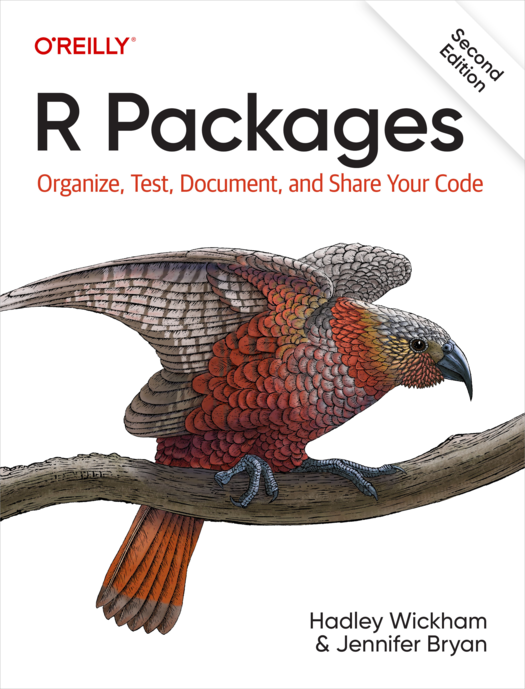
\includegraphics[width = 0.7\textwidth]{images/rpkgs-cover-2e-small.png}}
        \caption{%
          R Packages
        }
      \end{figure}%
    \end{column}
  \end{columns}
\end{frame}

\begin{frame}[c,fragile]
  \frametitle{Devtools}

  Meta-package for various helpers that
  aid in developing R packages (and projects).

  First off, install and load \textbf{devtools}:
  \begin{lstlisting}
        install.packages("devtools")
        library(devtools)
      \end{lstlisting}

  \begin{columns}
    \begin{column}{0.45\textwidth}

      This loads other packages that will be useful
      for setting up your package, most importantly the \textbf{usethis}
      package.
    \end{column}
    \begin{column}{0.45\textwidth}
      \begin{figure}[htpb]
        \centering
        
\includegraphics[width=2.5cm]{images/usethis-logo.png}%
        
\includegraphics[width=2.5cm]{images/devtools.pdf}
      \end{figure}
    \end{column}
  \end{columns}
\end{frame}

\begin{frame}[c]
  \frametitle{A Toy Example}

  \begin{block}{Rosenbrock Package}
    Let's build a simple package that solves the Rosenbrock optimization problem, i.e.
    find
    \[
      x^* = \operatorname{arg\,min}\left((a - x_1)^2 + b(x_2 - x_1^2)^2\right).
    \]
  \end{block}

  \bigskip\pause

  \begin{block}{What We Will Learn}
    \begin{itemize}[<+->]
      \item Adding R functions to our package
      \item Testing our code
      \item Interfacing with Rcpp
      \item Adding dependencies to other packages
      \item Licensing our package
      \item Documenting the code
    \end{itemize}
  \end{block}
\end{frame}

\begin{frame}[c,fragile]
  \frametitle{A First Package}
  \begin{block}{Create It}
    Call
    \begin{lstlisting}
          usethis::create_package("rosenbrock")
        \end{lstlisting}
    or use \texttt{File > New Project > New Directory > R Package using devtools} in R Studio.
  \end{block}

  \pause\bigskip

  \begin{columns}[T]
    \begin{column}{0.45\textwidth}
      Gives you a \alert{minimal} package:

      \medskip

      \dirtree{%
        .1 rosenbrock/.
        .2 R/.
        .2 DESCRIPTION.
        .2 NAMESPACE.
      }

      \medskip\pause

      You may also have \texttt{.Rbuildignore} and \texttt{.rosenbrock.Rproj}
      depending on how you created the package.
    \end{column}

    \pause

    \begin{column}{0.45\textwidth}
      \begin{block}{Install It}
        Open up the package in your editor (R Studio\footnote{In which case it
          should alread be opened.}).
        \begin{lstlisting}
          devtools::install()
        \end{lstlisting}

        \bigskip

        Voila, you have made an R package!
      \end{block}
    \end{column}
  \end{columns}

\end{frame}

\begin{frame}[c,fragile]
  \frametitle{R Code}

  \begin{block}{\texttt{.R/}}
    \begin{itemize}
      \item All R code should live in \texttt{.R}-files in \texttt{R/}.
      \item These files should (almost) always contain \alert{only} functions.
      \item Many ways to organize your files: one function per file, all functions
            of a certain S3 class in one file etc.
    \end{itemize}
  \end{block}

  \pause\bigskip

  Let's create a first file: \texttt{R/objective.R}. Use \lstinline{usethis::use_r("objective")} and insert this:

  \begin{lstlisting}
    objective <- function(x, a = 1, b = 100) {
      (a - x[1])^2 + b * (x[2] - x[1]^2)^2
    }
  \end{lstlisting}
\end{frame}

\begin{frame}[c,fragile]
  \frametitle{Workflow}
  We have created a first R file, but how do we use it? Two major options:

  \begin{columns}[T]
    \begin{column}{0.45\textwidth}
      \begin{block}{\lstinline{devtools::install()}}
        Installs the package, like calling \lstinline{install.packages()}.

        \medskip\pause

        Robust but slow. Need to call \lstinline{library(rosenbrock)}
        to load package\footnote{Done automatically in R Studio}.
      \end{block}
    \end{column}

    \pause

    \begin{column}{0.45\textwidth}
      \begin{block}{\lstinline{devtools::load_all()}}
        Sources all of your code.

        \medskip

        Quick but not as robust.

      \end{block}
    \end{column}
  \end{columns}

  \pause\bigskip

  \begin{block}{Try It}
    Try both options and see if you can call your newly defined function, \lstinline{objective()}.
  \end{block}
\end{frame}

\begin{frame}[c]
  \begin{figure}[htpb]
    \centering
    \frame{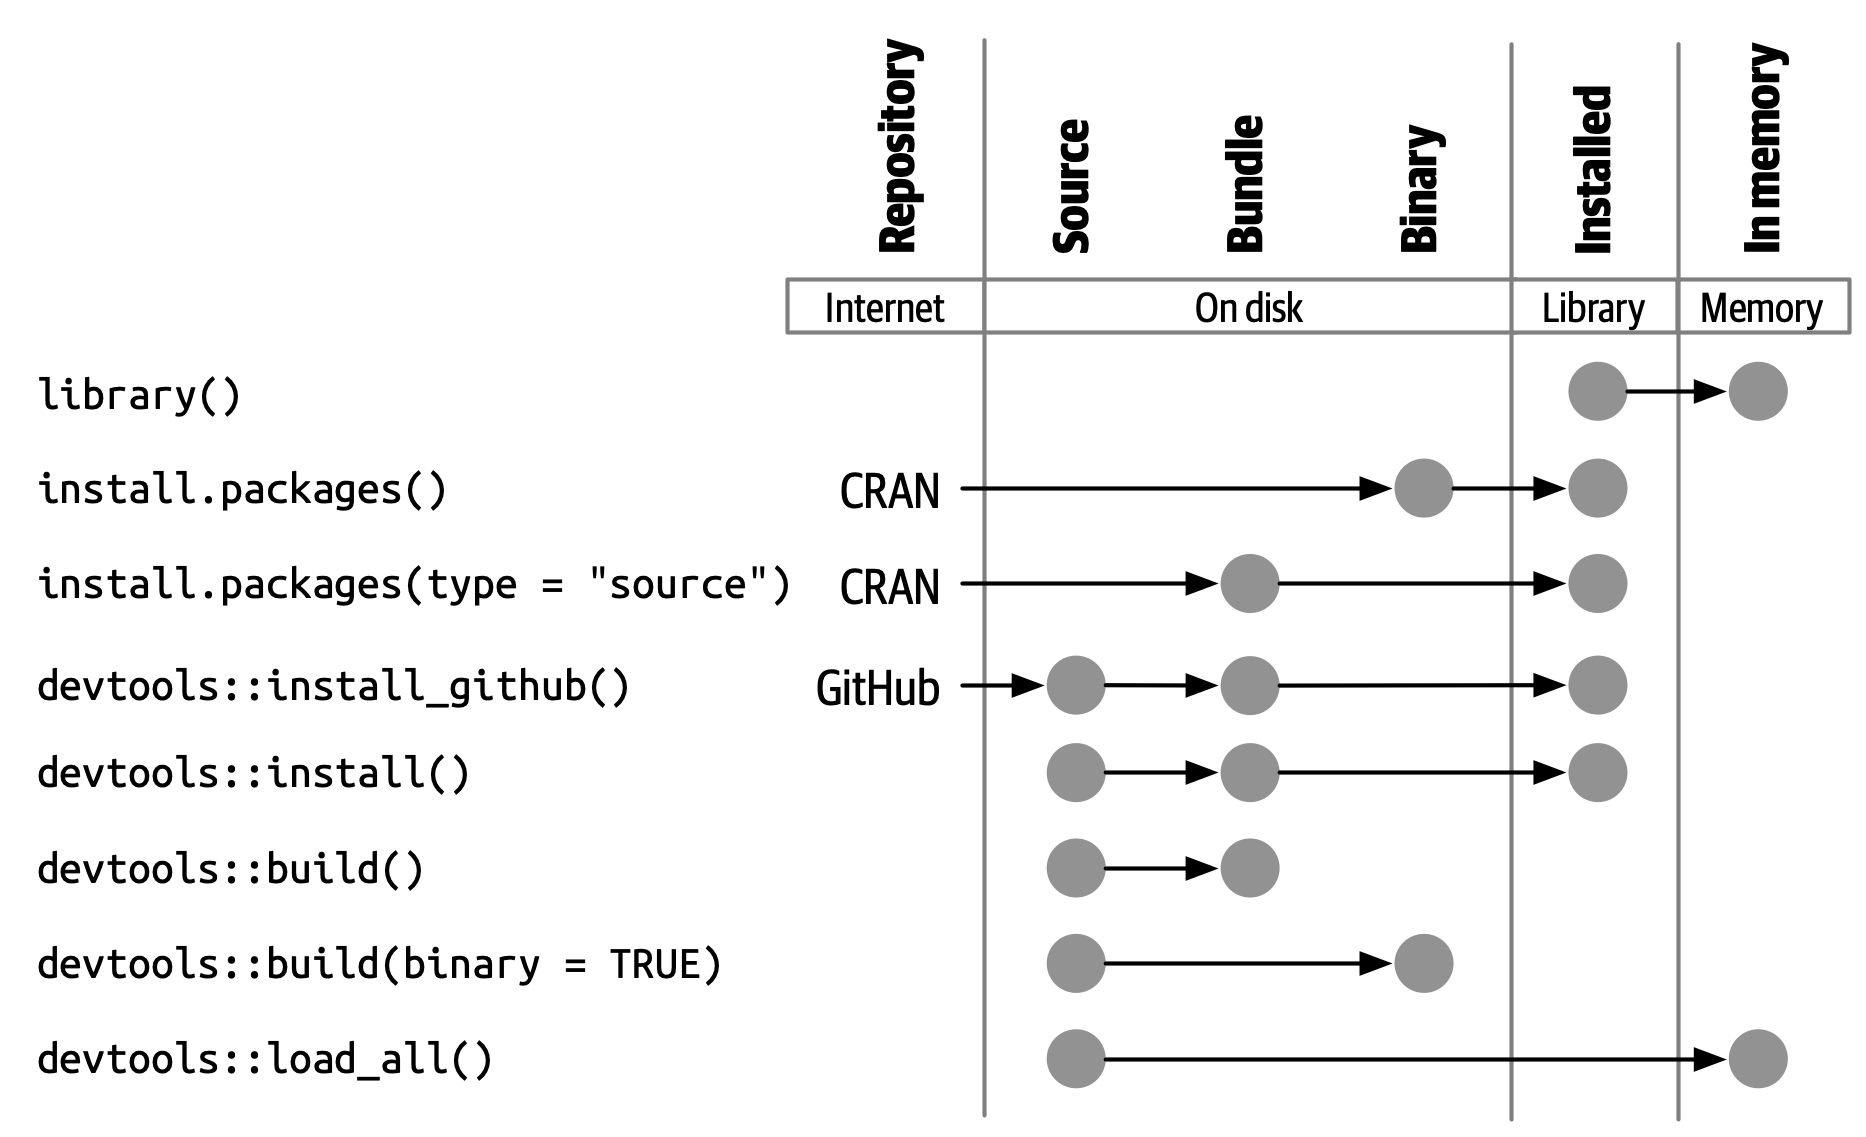
\includegraphics[width=0.92\textwidth]{images/install-load-states.png}}
    \caption{%
      The various states of a package and how to move between them.
    }
  \end{figure}
\end{frame}

\begin{frame}[c,fragile]
  \frametitle{Exporting Functions}

  If you called \lstinline{devtools::load_all()} then everything is sourced and you can
  just call \lstinline{objective()} directly.

  \bigskip

  But if you use \lstinline{devtools::install()} and \lstinline{library(rosenbrock)}, the
  you would need to use \lstinline{rosenbrock:::objective()}. The reason is that
  the function is not yet exported.

  \medskip\pause

  \begin{block}{\texttt{NAMESPACE}}

    Decides what functions you want exported. But right now it just contains a comment:
    \begin{lstlisting}
      # Generated by roxygen2: do not edit by hand
    \end{lstlisting}

    \pause\medskip

    If you want to just export everything, you can remove this file and recreate it with this content:
    \begin{lstlisting}
      exportPattern("^[[:alpha:]]+")
    \end{lstlisting}

  \end{block}
\end{frame}

\begin{frame}[c,fragile]
  \frametitle{roxygen2}

  \textbf{roxygen2} is a package that helps with package documentation\footnote{More on this later.},
  but it can also be used for handling the namespace.

  \bigskip\pause

  To export a function, you need to place a special roxygen2 comment just before the function:
  \begin{lstlisting}
    #' @export
  \end{lstlisting}

  \medskip\pause

  Go ahead and place this before your \lstinline{objective()} definition. Then run
  \lstinline{devtools::document()} to roxygenize your package.

  \bigskip\pause

  Now \texttt{NAMESPACE} will (should) contain this:
  \begin{lstlisting}
    export(objective)
  \end{lstlisting}

  \medskip\pause

  Reinstall the package and see if you can call \lstinline{objective()} after
  loading it.
\end{frame}

\begin{frame}[c,fragile]
  \frametitle{Tests}

  \begin{block}{testthat}
    \begin{itemize}
      \item We have already encountered \textbf{testthat} for writing tests in a formalized way.
      \item But \textbf{testthat} was actually written especially for packages.
    \end{itemize}
  \end{block}

  \pause\bigskip

  Let's start using \textbf{testthat} with our package:
  \begin{lstlisting}
    usethis::use_testthat()
  \end{lstlisting}

  \bigskip\pause

  This creates some new files and directories:

  \medskip

  \dirtree{%
    .1 rosenbrock/.
    .2 tests/.
    .3 testthat/.
    .4 test-<some\_fun>.R\DTcomment{Your test file for \texttt{some\_fun()}}.
    .3 testthat.R.
  }
\end{frame}

\begin{frame}[c,fragile]
  \frametitle{A First Simple Test}

  For the Rosenbrock function, \(f^* = f(a,a^2) = f(1,1) = 0\). Let's make sure this is the case for us too!

  \bigskip\pause

  To create a test, we can use \lstinline[basicstyle=\ttfamily]{usethis::use_test()}.

  \bigskip\pause

  Call \lstinline[basicstyle=\ttfamily]{use_test("objective")}\footnote<3->{It's good practice to name the test file the same as the file where the function you're testing is defined.} and insert this:
  \begin{lstlisting}
    test_that("multiplication works", {
      # add a test using expect_equal()
    })
  \end{lstlisting}

  \medskip\pause

  \begin{block}{Check That Everything Works}
    Run \lstinline[basicstyle=\ttfamily]{devtools::test()}, and hopefully see:

    \medskip

    \begin{lstlisting}
      [ FAIL 0 | WARN 0 | SKIP 0 | PASS 1 ]
    \end{lstlisting}
  \end{block}
\end{frame}

\begin{frame}[c]
  \frametitle{Checking}
  \begin{block}{\texttt{R CMD check}}
    R contains functionality for checking that your package is built correctly and you can
    access this functionality through \lstinline{devtools::check()}.
  \end{block}

  \bigskip\pause

  No requirement that your package needs to pass these checks (if you're using it as a project), but it's
  good practice to make sure it does.

  \bigskip\pause

  \begin{description}[<+->]
    \item[ERROR] Major problem with your package
    \item[WARNING] Something that is most likely not great but not critical
    \item[NOTE] Typically small issues with your package
  \end{description}

  \bigskip\pause

  Now run \lstinline{devtools::check()}. Is there a problem? Yes, let's fix it!

\end{frame}

\begin{frame}[c,fragile]
  \frametitle{Metadata}

  The metadata for your package lives in \texttt{DESCRIPTION}. Right now it looks like this:
  \begin{lstlisting}[basicstyle=\ttfamily\small]
    Package: rosenbrock
    Title: What the Package Does (One Line, Title Case)
    Version: 0.0.0.9000
    Authors@R:
        person("First", "Last", , "first.last@example.com", role = c("aut", "cre"),
               comment = c(ORCID = "YOUR-ORCID-ID"))
    Description: What the package does (one paragraph).
    License: `use_mit_license()`, `use_gpl3_license()` or friends to pick a
        license
    Encoding: UTF-8
    Roxygen: list(markdown = TRUE)
    RoxygenNote: 7.3.2
  \end{lstlisting}

  \pause\bigskip

  For now we'll leave most of these files alone, but let's
  fix one thing: the license
\end{frame}

\begin{frame}[c,fragile]
  \frametitle{Licensing}

  \begin{block}{Why Do You Need a License?}
    \begin{itemize}[<+->]
      \item Licensing software tells other people about how they are allowed to reuse your
            code.
      \item If you do not provide a license, this generally means that \alert{nobody is allowed to copy,
              distribute, or modify your code.}

      \item If you have other contributors, then ``nobody'' includes \alert{you too!}
    \end{itemize}

  \end{block}

  \pause

  \begin{block}{Choosing a License}
    So we need to pick a license: for now we'll pick the MIT license.\footnote<5->{Read more about picking a license at \url{https://choosealicense.com}.}

    \medskip\pause

    \begin{lstlisting}
      usethis::use_mit_license()
    \end{lstlisting}

    \medskip

    This will add new files to your package: \texttt{LICENSE}, \texttt{LICENSE.md}, and
    modify \texttt{DESCRIPTION}, in which you should see:

    \begin{lstlisting}
      License: MIT + file LICENSE
    \end{lstlisting}
  \end{block}
\end{frame}

\begin{frame}[c,fragile]
  \frametitle{Dependencies}

  In R packages, you make dependencies explicit, defined in \texttt{DESCRIPTION}

  \medskip\pause

  \begin{block}{Gradient}
    Let's say that we want to compute the gradient for the Rosenbrock function.

    \medskip\pause

    One way to do so is to use numerical differentiation through the \textbf{numDeriv} package:

    \begin{lstlisting}
      gradient <- function(x, a = 1, b = 100) {
        numDeriv::grad(objective, x, a = a, b = b)
      }
    \end{lstlisting}
  \end{block}

  Now our package depends on \textbf{numDeriv}, so we need to add it
  to \texttt{DESCRIPTION}:
  \begin{lstlisting}
    usethis::use_package("numDeriv")
  \end{lstlisting}

  \medskip\pause

  In \texttt{DESCRIPTION}, you should now see this:

  \begin{lstlisting}
    Imports: 
      numDeriv
  \end{lstlisting}

\end{frame}

\begin{frame}[c,fragile]
  \frametitle{Rcpp}

  \begin{columns}[T]
    \begin{column}{0.48\textwidth}

      Rcpp works best in a package:
      \begin{itemize}
        \item No more manual sourcing (no need to call \lstinline{Rcpp::sourceCpp()})
        \item You don't need to add directives for dependencies to \textbf{RcppArmadillo} and other
              packages.
      \end{itemize}

      \pause\medskip

      We will rely on \textbf{roxygen2}. First, call
      \begin{lstlisting}
        usethis::use_package_doc()
      \end{lstlisting}
      to set up a package doc file in \texttt{R/rosenbrock-package.R}.
    \end{column}

    \pause

    \begin{column}{0.42\textwidth}
      Then use \lstinline{usethis::use_rcpp()} to put the pieces in place:

      \medskip

      \dirtree{%
        .1 rosenbrock/.
        .2 src/.
        .3 slop-package.cpp/.
      }

      \medskip\pause

      Now just need to run \texttt{devtools::document()} and
      \lstinline{devtools::load_all()} or \lstinline{devtools::install()}
      and now your code is available (but not exported).
    \end{column}
  \end{columns}

\end{frame}

\begin{frame}[c,fragile]
  \frametitle{Exporting Rcpp Code}
  \begin{columns}[T]
    \begin{column}{0.45\textwidth}
      \begin{block}{Wrapping}
        Call your Rcpp function through an R wrapper:
        \begin{lstlisting}
          my_fun <- function(x) {
            my_fun_cpp(x)
          }
        \end{lstlisting}

        \pause

        Typically easier because checking input and preparing output is
        easier on the R side.
      \end{block}
    \end{column}\pause
    \begin{column}{0.45\textwidth}
      \begin{block}{Direct Export}
        You can add roxygen2 comments in Rcpp code too:
        \begin{lstlisting}[language=C++]
          //' @export
          double my_fun_cpp() {...}
        \end{lstlisting}

        \pause

        Saves you having to write and maintain an R function.
      \end{block}
    \end{column}
  \end{columns}
\end{frame}

\begin{frame}[c]
  \frametitle{Documentation}

  \begin{columns}[T]
    \begin{column}{0.45\textwidth}
      \begin{block}{Why?}
        Because
        \begin{itemize}[<+->]
          \item you make your code accessible to others,
          \item it makes you think an extra time about what your function is doing, and
          \item your future self will thank you.
        \end{itemize}
      \end{block}
    \end{column}
    \medskip\pause

    \begin{column}{0.45\textwidth}
      \begin{block}{Types}
        \begin{itemize}
          \item Comments in code
          \item Manual (help files)
          \item Long-form articles (vignettes)
        \end{itemize}
      \end{block}
    \end{column}
  \end{columns}

  \begin{block}{roxygen2}
    Primary purpose of the package. You write code is a special syntax
    and it converts it into manual files that R understands.
  \end{block}

\end{frame}

\begin{frame}[c,fragile]
  \frametitle{roxygen2 Syntax}
  \begin{lstlisting}
    #' Function Title
    #' 
    #' Here you describe what the function does, possibly 
    #' using several lines.
    #' 
    #' @param x Explanation of argument x
    #'
    #' @return Explanation of what the function returns
    #'
    #' @export
    my_fun <- function(x) {
      ...
    }
  \end{lstlisting}

  \pause

  \begin{block}{Your Turn}
    Document \lstinline{objective()} with roxygen2 syntax. No need for
    sensible documentation. Just make sure you have the bare minimum.
  \end{block}

\end{frame}

\begin{frame}[c]
  \frametitle{Documentation in This Course}

  \begin{itemize}
    \item Not making a package for CRAN, so lower standards.
    \item You don't need to document to benefit from building a package.
    \item But it's not a bad idea to do so anyway!
  \end{itemize}
\end{frame}

\begin{frame}[c]
  \begin{figure}[htpb]
    \centering
    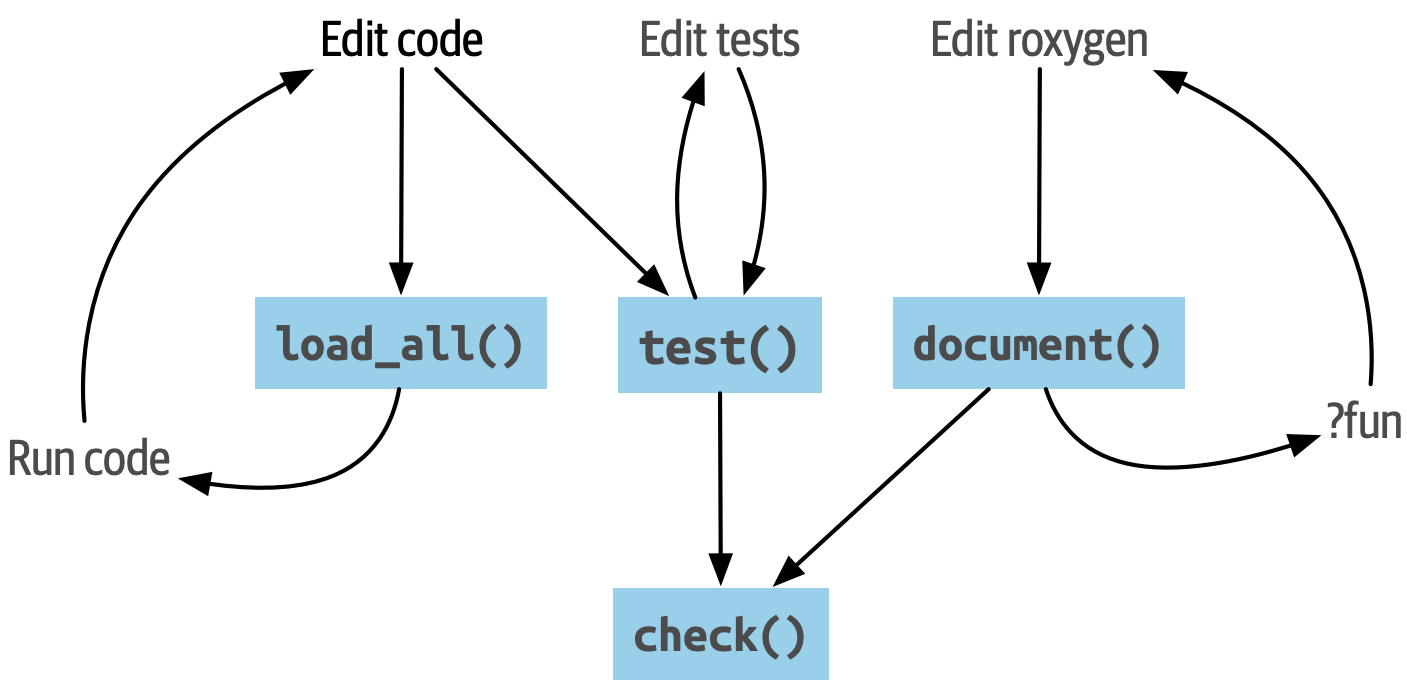
\includegraphics[width=0.9\textwidth]{images/pkgs-workflow.png}
    \caption{%
      The whole game
    }
  \end{figure}
\end{frame}

\begin{frame}[c]
  \frametitle{Projects}

  When you have a project, you typically need more things:
  \begin{itemize}
    \item scripts with simulations, etc, which produce output
    \item datasets stored in different formats
    \item notebooks (or latex sources)
  \end{itemize}

  These things do not naturally fit into a package framework.

  \pause

  \begin{block}{Two Choies of Structure}
    \begin{enumerate}[<+->]
      \item Just store these things directly into the package folder. Optionally, you can use \texttt{.Rbuildignore}
            to ignore these files when building the package.
      \item Put your \textbf{package} into a \alert{subdirectory} of your project. This cleanly separates
            the part of your project that contains reusable code (the package) and the
            part that is experiments and reports. But a little trickier to setup.
    \end{enumerate}

  \end{block}

\end{frame}

\begin{frame}[c]
  \frametitle{Exercise: Two Options}

  \begin{block}{Rosenbrock}
    Continue building the \textbf{rosenbrock} package:
    \begin{itemize}[<+->]
      \item Write a gradient descent (or stochastic gradient descent) implementation that
            minimizes the rosenbrock function.
      \item Write the code in Rcpp. If you want, you can first write it in R to
            see that everything is working, and then port it.
      \item Feel free to use generative AI to write the code.
      \item Export everything and document the package.
    \end{itemize}
  \end{block}

  \pause

  \begin{block}{An Assignment}
    Start trying to convert your work for one assignment into a package
  \end{block}
\end{frame}

\begin{frame}[c]
  \frametitle{What We Didn't Cover}

  \begin{itemize}[<+->]
    \item Version control through git and github
    \item How to properly format metadata (\texttt{DESCRIPTION})
    \item Integrating data into our package
    \item Publishing to CRAN
    \item Principled approaches to reproducibility (renv, containers)
  \end{itemize}

\end{frame}

\section{Oral Examination Prep}

\begin{frame}[c]
  \frametitle{Procedure}
  \begin{enumerate}[<+->]
    \item After entering the room you will connect the computer and check that
          it works with the projector.
    \item When all technical issues are settled,
          you will draw the assignment and find the presentation on the computer.
    \item Time starts and you have 15 min for the presentation. The examiners
          may ask questions if something needs to be clarified.
    \item After 15 min
          your presentation will be stopped, and the examiners will ask questions
          related to the assignment as well as to the general content of the
          course.
    \item After at most 25 min the exam ends, and after assessment
          you will be given a grade.
  \end{enumerate}

  \pause

  \begin{block}{Examiners}
    Me and Jonas Gyde Hermansen

    \medskip

    It's possible that Niels will show up during one or two of the examinations.
  \end{block}

\end{frame}

\begin{frame}[c]
  \frametitle{The Five Points}

  \begin{block}{Remember the Five Points}
    \begin{itemize}[<+->]
      \item How can you test that your implementation is correct?
      \item Can you implement alternative solutions?
      \item Can the code be restructured e.g. by modularization, abstraction or object oriented programming to improve generality, extendability and readability?
      \item How does the implementation perform (benchmarking)?
      \item Where are the bottlenecks (profiling), and what can you do about them?
    \end{itemize}
  \end{block}
\end{frame}

\begin{frame}[c]
  \frametitle{Advice}

  \begin{itemize}[<+->]
    \item You \alert{only} have 15 minutes.
    \item Focus on aspects of the problem you thought were interesting.
    \item You aren't expected to have covered every aspect of the problem in depth.
    \item Try to tell a story about what you tried, what didn't work, and why
          you settled for a particular solution.
    \item Use plots as much as possible
    \item Good to include math and code, but avoid overwhelming us.
  \end{itemize}
\end{frame}

\begin{frame}[c]
  \frametitle{Evaluation Criteria}

  \begin{block}{Knowledge}
    Knowledge of fundamental algorithms for statistical computations and R packages that implement some of these algorithms or are useful for developing novel implementations.
  \end{block}

  \pause
  \begin{block}{Skills}
    Ability to implement, test, debug, benchmark, profile and optimize statistical software.
  \end{block}

  \pause

  \begin{block}{Competence}
    Ability to select appropriate numerical algorithms for statistical computations and
    evaluate implementations in terms of correctness, robustness, accuracy and memory and speed efficiency.
  \end{block}

\end{frame}

\section{Course Summary}

\begin{frame}[c]
  \frametitle{Course Summary}

  \begin{block}{Statistical Topics}
    \begin{description}[<+->][Optimization]
      \item[Smoothing] Kernel density smoothing and splines (topic 1)
      \item[Simulation] MC methods: rejection and importance sampling (topic 2)
      \item[Optimization] The EM algorithm (topic 3), gradient descent and stochastic optimization (topic 4)
    \end{description}
  \end{block}

  \pause

  \begin{block}{Computational Topics}
    \begin{itemize}
      \item Debugging
      \item Profiling
      \item Benchmarking
      \item Debugging
      \item Writing performant code
    \end{itemize}
  \end{block}
\end{frame}

\begin{frame}[standout]
  Thank you!
\end{frame}

% \appendix

% \begin{frame}[allowframebreaks]{References}
%   \printbibliography[heading=none]
% \end{frame}


\end{document}

